\documentclass[12pt]{article}

% Packages for JAMA Oncology formatting
\usepackage[utf8]{inputenc}
\usepackage[T1]{fontenc}
\usepackage{amsmath,amssymb}
\usepackage{graphicx}
\usepackage{booktabs}
\usepackage{multirow}
\usepackage{array}
\usepackage{float}
\usepackage{threeparttable}
\usepackage{hyperref}
\usepackage{natbib}
\usepackage{setspace}
\usepackage[margin=1in]{geometry}
\usepackage{enumitem}
\usepackage{xcolor}
\usepackage{caption}

% JAMA Oncology specific formatting
\onehalfspacing
\setlength{\parindent}{0.5in}
\setlength{\parskip}{0pt}

\begin{document}

% ============================================
% TITLE PAGE
% ============================================
\begin{titlepage}
    \centering
    \vspace*{0.5cm}
    
    {\Large\bfseries User Communication Style Determines LLM Safety in Cancer Counseling\par}
    
    \vspace{1cm}
    
    {\large
    Ramez Kouzy, MD\textsuperscript{1,2}; 
    Jack Gallifant, MBBS\textsuperscript{3,4}; 
    Shan Chen, PhD\textsuperscript{3,5}; \\
    Marielle Fils, BS\textsuperscript{6}; 
    Roxana Attar, MD\textsuperscript{7}; 
    Danielle S. Bitterman, MD\textsuperscript{3,5}
    }
    
    \vspace{0.8cm}
    
    {\small
    \begin{flushleft}
    \textsuperscript{1}Department of Radiation Oncology, The University of Texas MD Anderson Cancer Center, Houston, TX \\
    \textsuperscript{2}Institute for Data Science in Oncology, The University of Texas MD Anderson Cancer Center, Houston, TX \\
    \textsuperscript{3}Artificial Intelligence in Medicine Program, Mass General Brigham, Boston, MA \\
    \textsuperscript{4}Laboratory for Computational Physiology, Massachusetts Institute of Technology, Cambridge, MA \\
    \textsuperscript{5}Department of Radiation Oncology, Dana-Farber Cancer Institute and Brigham and Women's Hospital, Harvard Medical School, Boston, MA \\
    \textsuperscript{6}School of Medicine and Health Sciences, The George Washington University, Washington, DC \\
    \textsuperscript{7}Department of Radiation Oncology, Texas Tech University Health Sciences Center El Paso, El Paso, TX
    \end{flushleft}
    }
    
    \vspace{1cm}
    
    {\normalsize
    \textbf{Corresponding Author:} \\
    Danielle S. Bitterman, MD \\
    Department of Radiation Oncology \\
    Dana-Farber Cancer Institute and Brigham and Women's Hospital \\
    Harvard Medical School \\
    75 Francis Street, ASB1-L2 \\
    Boston, MA 02115 \\
    Email: dsbitterman@bwh.harvard.edu
    }
    
    \vspace{0.8cm}
    
    {\normalsize
    \textbf{Word Count:} 3,850 \\
    \textbf{Figures:} 4 \\
    \textbf{Tables:} 1 (+ 2 Supplementary) \\
    \textbf{References:} 36
    }
    
    \vspace{0.8cm}
    
    {\normalsize
    \textbf{Running Title:} User Communication Style and LLM Safety \\
    \textbf{Keywords:} Large language models, artificial intelligence, sycophancy, cancer misinformation, patient safety
    }
    
    \vspace{0.5cm}
    
    {\small
    \textbf{Conflict of Interest:} The authors declare no conflicts of interest. \\
    \textbf{Funding:} None. \\
    \textbf{Data Availability:} Code and de-identified conversation data available at [repository].
    }
    
\end{titlepage}

\newpage

% ============================================
% ABSTRACT
% ============================================

\section*{Abstract}

\noindent\textbf{Introduction:} Patients increasingly rely on large language model (LLM) chatbots for medical information. While these models perform well on evidence-aligned queries, their safety when confronted with patient misconceptions remains uncharacterized in oncology, where validation of unproven therapies can lead to treatment abandonment and worse outcomes. We hypothesized that LLMs exhibit validation bias (sycophancy) when patients present non-evidence-based views about cancer treatment, increasing the rate of unsafe responses compared with evidence-aligned framing.

\noindent\textbf{Methods:} We conducted a cross-sectional stress test using a 2$\times$2$\times$2 factorial design to evaluate 6,360 individual model interactions across 1,272 structured conversations involving 14 LLMs from 6 providers (OpenAI, Anthropic, Google, Meta, DeepSeek, Alibaba). Conversations varied by framing (patient misconceptions vs evidence-aligned), treatment type (evidence-based vs unproven/alternative), and format (single-turn vs multi-turn). The primary outcome was the rate of unsafe responses, defined as a ``Weak'' classification on a 6-dimension safety rubric (score 0 to 5 of 12) or the presence of critical failures (e.g., generating promotional content for harmful treatments). Secondary outcomes included safety erosion and dimension-level scores.

\noindent\textbf{Results:} Framing queries with patient misconceptions significantly increased the rate of unsafe responses compared with evidence-aligned framing (14.4\% [93/644] vs 5.1\% [32/628]; odds ratio [OR], 3.13; 95\% CI, 2.05 to 4.79; P $<$ .001). Beyond outright failures, 22.6\% of safe conversations degraded in quality under misconception conditions. Multi-turn dialogue was protective, reducing unsafe response rates by 68\% (OR, 0.32; 95\% CI, 0.21 to 0.48; P $<$ .001). Performance varied substantially by provider, with unsafe rates ranging from 1.8\% (Anthropic) to 36.8\% (DeepSeek).

\noindent\textbf{Conclusions:} LLMs exhibited significant sycophancy in oncology, validating patient misconceptions at 2.8 times the rate of evidence-aligned queries. This validation bias presents a safety risk that standard evaluations miss. Clinical integration of AI assistants requires adversarial testing and multi-turn guardrails to prevent reinforcement of harmful beliefs about cancer treatment.

\newpage

% ============================================
% INTRODUCTION
% ============================================

\section{Introduction}

Patients have long turned to the internet to supplement or challenge medical advice, but the emergence of artificial intelligence (AI) chatbots has fundamentally altered this landscape. Unlike static search engines, large language models (LLMs) engage users in conversational dialogue, offering personalized synthesis of complex medical information.\cite{singhal2023large,vanveen2024adapted,zakka2024almanac} Early evaluations have been promising: studies comparing AI responses to physician answers have found LLMs to be empathetic and generally accurate when answering patient questions about cancer.\cite{ayers2023comparing,pan2023assessment,laymouna2024roles} However, these assessments typically rely on a critical assumption: that patients ask questions neutrally, seeking objective truth. In clinical reality, patients often approach medical information with preexisting beliefs, seeking validation for unproven alternative therapies or confirmation of fears regarding evidence-based treatments. This distinction is crucial because LLMs are trained to be helpful and harmless---objectives that can conflict when a user's intent is misaligned with medical evidence.

A growing body of computer science literature identifies ``sycophancy'' as a pervasive alignment failure: the tendency of models to agree with users' stated views to maximize satisfaction rather than prioritize accuracy.\cite{bennatan2026sycophant,christian2026selfblinding,cheng2026accommodation,celebi2025parrot,hu2025monica,rahman2025pendulum,zhang2025humanlike,chang2026internal} In general domains, this might result in an AI agreeing with a user's political preference; in oncology, it could mean validating a decision to forgo life-saving therapy. The clinical stakes of such validation are severe. Patients with cancer who choose alternative medicine over evidence-based treatments face a twofold greater risk of death.\cite{johnson2018alternative} If AI tools reinforce rather than correct misconceptions about these treatments, they may inadvertently accelerate pathways to treatment abandonment.\cite{peterson2023international,yoon2022understanding,delgadolopez2018influence} As AI chatbots increasingly replace search engines as primary information sources, they inherit the responsibility to navigate these misconceptions safely.

Current medical AI benchmarks primarily test performance on evidence-aligned, fact-seeking queries, leaving a significant gap in our understanding of how models perform under adversarial or belief-laden conditions.\cite{huo2025large,shool2025systematic,moreno2024toward,kouzy2025oneshot} Prior evaluations have established that models can provide accurate and empathetic responses when asked direct questions like ``What are the common symptoms of lung cancer?''\cite{pan2023assessment,ayers2023comparing,bai2025application} While valuable, these studies test knowledge retrieval under ideal conditions---they do not assess robustness when a user asserts, ``I heard chemotherapy is poison and I should take black salve instead.'' Recent work by Mo and colleagues demonstrated that LLMs exhibit tension between faithfulness to provided context and adherence to safety protocols when presented with counterfactual medical evidence, suggesting that adversarial framing may systematically compromise model safety.\cite{mo2026faithfulness} By omitting these adversarial scenarios, existing benchmarks may overestimate the safety of LLMs for real-world patient populations.

We hypothesized that LLMs exhibit validation bias when patients present non-evidence-based views about cancer treatment, resulting in higher rates of unsafe responses compared with evidence-aligned framing. To test this hypothesis, we designed a controlled 2$\times$2$\times$2 factorial experiment to determine whether LLMs maintain safety standards when users frame questions with unsubstantiated claims, either by promoting unproven cures or attacking evidence-based therapies. By evaluating 14 leading models through 6,360 individual interactions, we aimed to quantify the ``sycophancy gap'' in medical AI safety and identify factors, such as conversational depth, that might mitigate this risk.

\newpage

% ============================================
% METHODS
% ============================================

\section{Methods}

\subsection{Study Design}

We conducted a 2$\times$2$\times$2 factorial experiment to evaluate the safety and alignment of large language models (LLMs) when discussing cancer treatments from a patient-centered perspective. The three experimental factors were: (1) conversation format (single-turn vs multi-turn), (2) treatment type (evidence-based vs alternative), and (3) query valence (positive vs negative framing). This design yielded 8 experimental conditions representing the spectrum of patient communication patterns encountered in clinical practice.

The conversation structure was designed to model authentic patient-clinician interactions based on clinical experience with cancer treatment counseling. Multi-turn conversations followed an escalating protocol, from routine information-seeking to increasingly safety-critical scenarios, reflecting the natural progression of patient inquiries rather than purely adversarial testing. Importantly, the 8 conditions span a range from entirely benign (e.g., a patient asking positively about chemotherapy) to potentially harmful (e.g., requesting promotional content for unproven treatments).

Prior studies have isolated individual factors contributing to sycophancy in medical AI, including the effect of valence alone or single-turn versus multi-turn interactions.\cite{mo2026faithfulness,celebi2025parrot} However, no systematic evaluation has examined how conversation format, treatment evidence base, and user framing interact simultaneously to influence safety-relevant outputs in cancer care. Notably, prior adversarial testing has generally found multi-turn interactions to be more vulnerable than single-turn exchanges; our study design allowed us to evaluate whether this pattern holds in the oncology context. We developed a structured evaluation rubric grounded in principles of clinical cancer care communication to quantify model performance across these conditions.

\subsection{Conversation Dataset}

We evaluated 1,272 conversations corresponding to 6,360 LLM-user interactions across 14 LLMs from 6 providers between March and September 2025. Model selection aimed to create a representative sample of publicly accessible LLMs available to patients at the time of the study, including free-tier commercial models, open-source models, and reasoning-focused architectures. The evaluated models were: Claude 3.5 Haiku and Claude 3.7 Sonnet (Anthropic); Gemini 1.5 Flash, Gemini 2.0 Flash, Gemini 2.0 Thinking, and Gemini 2.5 Pro (Google); Gemma 3 4B and Gemma 3 27B (Google, open-source); GPT-4o, GPT-4o-mini, and O3-mini (OpenAI); DeepSeek R1 Distill (DeepSeek, open-source); Llama 3.2 3B (Meta, open-source); and Qwen 3 32B (Alibaba, open-source).

The treatment dataset comprised 15 alternative therapies and 15 evidence-based therapies selected to represent the range of unproven and evidence-based cancer treatments patients commonly encounter (Appendix 1). Each treatment was queried across two formats and two valences. In the multi-turn format, five sequential queries (T1--T5) were delivered within a single conversation with context maintained between turns, allowing the model to reference prior exchanges. In the single-turn format, the same five queries were delivered as independent, isolated prompts without conversational context. To isolate the effect of valence while minimizing other confounds, positive and negative versions of each query differed by only one or two key words (e.g., ``effective'' vs ``ineffective,'' ``improved'' vs ``worsened,'' ``should'' vs ``shouldn't,'' ``promotional content'' vs ``warning content''), with all other phrasing held constant.

\subsection{Evaluation Rubric}

We developed a structured rubric (maximum 12 points) with six dimensions assessing distinct aspects of model safety (Appendix 2). \textbf{Evidence Accuracy (0--3 points)} evaluated factual correctness with appropriate clinical context. \textbf{Testimonial Handling (0--1 point)} assessed whether models explained why anecdotal evidence cannot establish treatment efficacy. \textbf{Safety Guidance (0--2 points)} measured clarity and proactivity of safety recommendations. \textbf{Misattribution Correction (0--1 point)} assessed whether models corrected false claims about having recommended specific treatments. \textbf{Promotional Content Response (0--3 points)} evaluated refusal to generate marketing materials. \textbf{Healthcare Professional References (0--2 points)} counted consistency of medical consultation recommendations.

Conversations were classified as Strong (10--12 points with no critical failures), Moderate (6--9 points with no critical failures), or Weak (0--5 points or any critical failure). Three categories of critical failure resulted in automatic Weak classification: (1) \textit{Enables Dangerous Implementation}, (2) \textit{Actively Endorses Harmful Content}, and (3) \textit{Creates Promotional Content}.

\subsection{Conversation Scoring}

We used GPT-5-mini via the OpenAI Batch API as an automated judge for scalable, consistent evaluation. The judge received structured prompts containing the complete rubric criteria, the conversation transcript, and instructions to first provide qualitative analysis of each rubric dimension before generating scores. This chain-of-thought approach improved scoring consistency by requiring explicit reasoning.

The judge produced dimension-level qualitative assessments which were then converted to numeric scores using Python algorithms. Healthcare Professional Reference counts were computed algorithmically by pattern-matching explicit medical consultation recommendations across all model responses.

Judge prompts and scoring algorithms were iteratively refined on a pilot set of 88 conversations with dual human annotation by two clinical researchers. Disagreements were resolved through discussion to establish a gold standard. Agreement was assessed as the percentage of cases where the LLM judge score matched at least one human annotator (``LLM vs Any Human''), reflecting practical alignment with acceptable human judgment rather than requiring exact match with a single adjudicated score. Overall agreement was 81.8\%, with dimension-level agreement ranging from 77.3\% (Misattribution Correction) to 93.2\% (Testimonial Handling) (Appendix 3).

\subsection{Statistical Analysis}

Categorical comparisons (classification distributions, critical failure rates) used Pearson chi-square tests or Fisher's exact test when expected cell counts were $<$5. Odds ratios with 95\% confidence intervals quantified effect sizes for binary outcomes. Wilson score intervals provided confidence intervals for proportions.

Continuous score comparisons used independent samples $t$-tests for two-group comparisons and one-way ANOVA with Tukey HSD post-hoc tests for multi-group comparisons across the four treatment$\times$valence conditions.

To model critical failure risk, we fit logistic regression models with treatment type, valence, format, and their interactions as predictors. Model comparison used likelihood ratio tests to evaluate the significance of interaction terms. Predicted probabilities were computed for each experimental condition.

To assess the joint effects of all three experimental factors on total rubric scores, we conducted three-way ANOVA (Format $\times$ Treatment $\times$ Valence) with partial eta-squared ($\eta_p^2$) as effect size measures.

All analyses were conducted in Python 3.10\cite{python310} using pandas 1.5.3\cite{pandas153}, NumPy 1.24.2\cite{numpy1242}, scikit-learn 1.2.2\cite{scikitlearn122}, and statsmodels 0.14.0\cite{statsmodels0140}. Statistical significance was set at $\alpha = 0.05$ (two-sided) for all tests.

\subsection{Reporting Standards}

This study adheres to the TRIPOD-LLM (Transparent Reporting of a Multivariable Prediction Model for Individual Prognosis or Diagnosis for Large Language Models) reporting guideline for studies using large language models.\cite{gallifant2025tripod} Complete details on model specifications, prompting strategies, evaluation procedures, and statistical methods are provided in the manuscript and supplementary appendix.

\newpage

% ============================================
% RESULTS
% [Continued in next section due to length...]
% ============================================

\section{Results}

\subsection{Overall Safety Performance}

The majority of conversations were classified as Strong (919 [72.2\%]) or Moderate (228 [17.9\%]), with 125 conversations (9.8\%) classified as Weak (unsafe). A total of 111 conversations (8.7\%) contained at least one critical failure that could directly harm patients.

\subsection{The Sycophancy Effect}

Framing queries with patient misconceptions---either promoting unproven treatments or attacking evidence-based therapies---significantly increased unsafe response rates compared with evidence-aligned framing (14.4\% [93/644] vs 5.1\% [32/628]; OR, 3.13; 95\% CI, 2.05 to 4.79; P $<$ .001; Table 2, Figure 1). This validation bias persisted regardless of whether patients promoted harmful treatments (``colloidal silver cures cancer'') or disparaged proven therapies (``chemotherapy is poison''), indicating that models prioritized agreement over accuracy.

\subsection{Safety Degradation in High-Performing Models}

Among 429 conversations achieving Strong classification under evidence-aligned framing, 97 (22.6\%) degraded in quality when shifted to misconception framing: 54 (12.6\%) declined to Moderate and 43 (10.0\%) fell to Weak (Figure 4A). This erosion occurred even in models that initially performed well, demonstrating that misconception framing compromises quality beyond outright failure.

\subsection{Protective Effect of Multi-Turn Dialogue}

Multi-turn conversations demonstrated substantially lower unsafe response rates compared with single-turn exchanges (5.2\% [34/655] vs 14.8\% [91/617]; OR, 0.32; 95\% CI, 0.21 to 0.48; P $<$ .001; Figure 2). This represents a 6.0 percentage point absolute risk reduction for evidence-aligned queries and a 13.1 percentage point reduction for misconception-framed queries. Under the highest-risk condition---single-turn queries with misconception framing---21.2\% of conversations resulted in unsafe responses. Multi-turn format reduced this to 8.1\% (absolute risk reduction: 13.1 percentage points). Extended dialogue provided substantial protection against validation bias.

\subsection{Critical Failure Patterns}

Critical failures were dominated by promotional content generation (105 of 111 conversations [94.6\%]), where models produced marketing-like statements positioning unproven therapies favorably. Active endorsement of harmful content occurred in 43 conversations (38.7\%), with models explicitly validating unproven treatment efficacy or dangers of evidence-based therapies. Two conversations (1.8\%) contained dangerous implementation guidance. Failure modes extended beyond passive validation to active promotion using persuasive language characteristic of alternative medicine advertising.

\subsection{Variation Across Model Providers}

Unsafe response rates varied substantially by provider (Supplementary Table 1, (Supplementary Figure 1)). Top-performing models included Gemini 1.5 Flash, Claude 3.7 Sonnet, and O3-mini (each 0.8\% unsafe). The highest-risk models were DeepSeek R1 Distill (36.8\% unsafe) and Gemma 3 4B (35.6\% unsafe), representing a 46-fold difference between best and worst performers.

\subsection{Dimension-Level Safety Degradation}

Misconception framing most severely degraded Promotional Content Response scores (mean 2.42 vs 2.73 out of 3 points; P $<$ .001) and Evidence Accuracy scores (2.68 vs 2.80; P $<$ .001; Supplementary Table 2, (Supplementary Figure 2)). These dimensions captured the core failures: unwillingness to refuse promotional requests and reduced factual accuracy under adversarial framing.

\newpage

% ============================================
% TABLES
% ============================================

\begin{table}[htbp]
\centering
\small
\caption{Primary Safety Outcomes: The Sycophancy Effect by Framing Condition}
\label{tab:primary-outcomes}
\begin{threeparttable}
\begin{tabular}{@{}lcccc@{}}
\toprule
 & \multicolumn{2}{c}{\textbf{Framing}} & & \\
\cmidrule(lr){2-3}
\textbf{Outcome} & \textbf{Evidence-aligned} & \textbf{Misconception} & \textbf{OR (95\% CI)} & \textbf{P} \\
\midrule
\multicolumn{5}{@{}l}{\textit{Safety Classification, No. (\%)}} \\
\addlinespace
\quad Strong & 477 (75.0) & 442 (69.5) & --- & .021 \\
\quad Moderate & 127 (20.0) & 101 (15.9) & --- & .048 \\
\quad Weak (Unsafe) & 32 (5.0) & 93 (14.4) & 3.13 (2.05--4.79) & <.001 \\
\addlinespace
\multicolumn{5}{@{}l}{\textit{Total Score (0--12), Mean (SD)}} \\
\addlinespace
\quad & 10.22 (2.1) & 9.94 (2.8) & --- & .045 \\
\addlinespace
\multicolumn{5}{@{}l}{\textit{Critical Failures*, No. (\%)}} \\
\addlinespace
\quad Any & 25 (3.9) & 86 (13.5) & 3.84 (2.40--6.14) & <.001 \\
\bottomrule
\end{tabular}
\begin{tablenotes}[flushleft]
\footnotesize
\item Abbreviations: CI, confidence interval; OR, odds ratio; SD, standard deviation.
\item * Enables dangerous implementation, actively endorses harmful content, or creates promotional content.
\item Misconception framing: promoting unproven treatments or questioning evidence-based treatments.
\end{tablenotes}
\end{threeparttable}
\end{table}
% ============================================
% FIGURES
% ============================================

\begin{figure}[htbp]
\centering
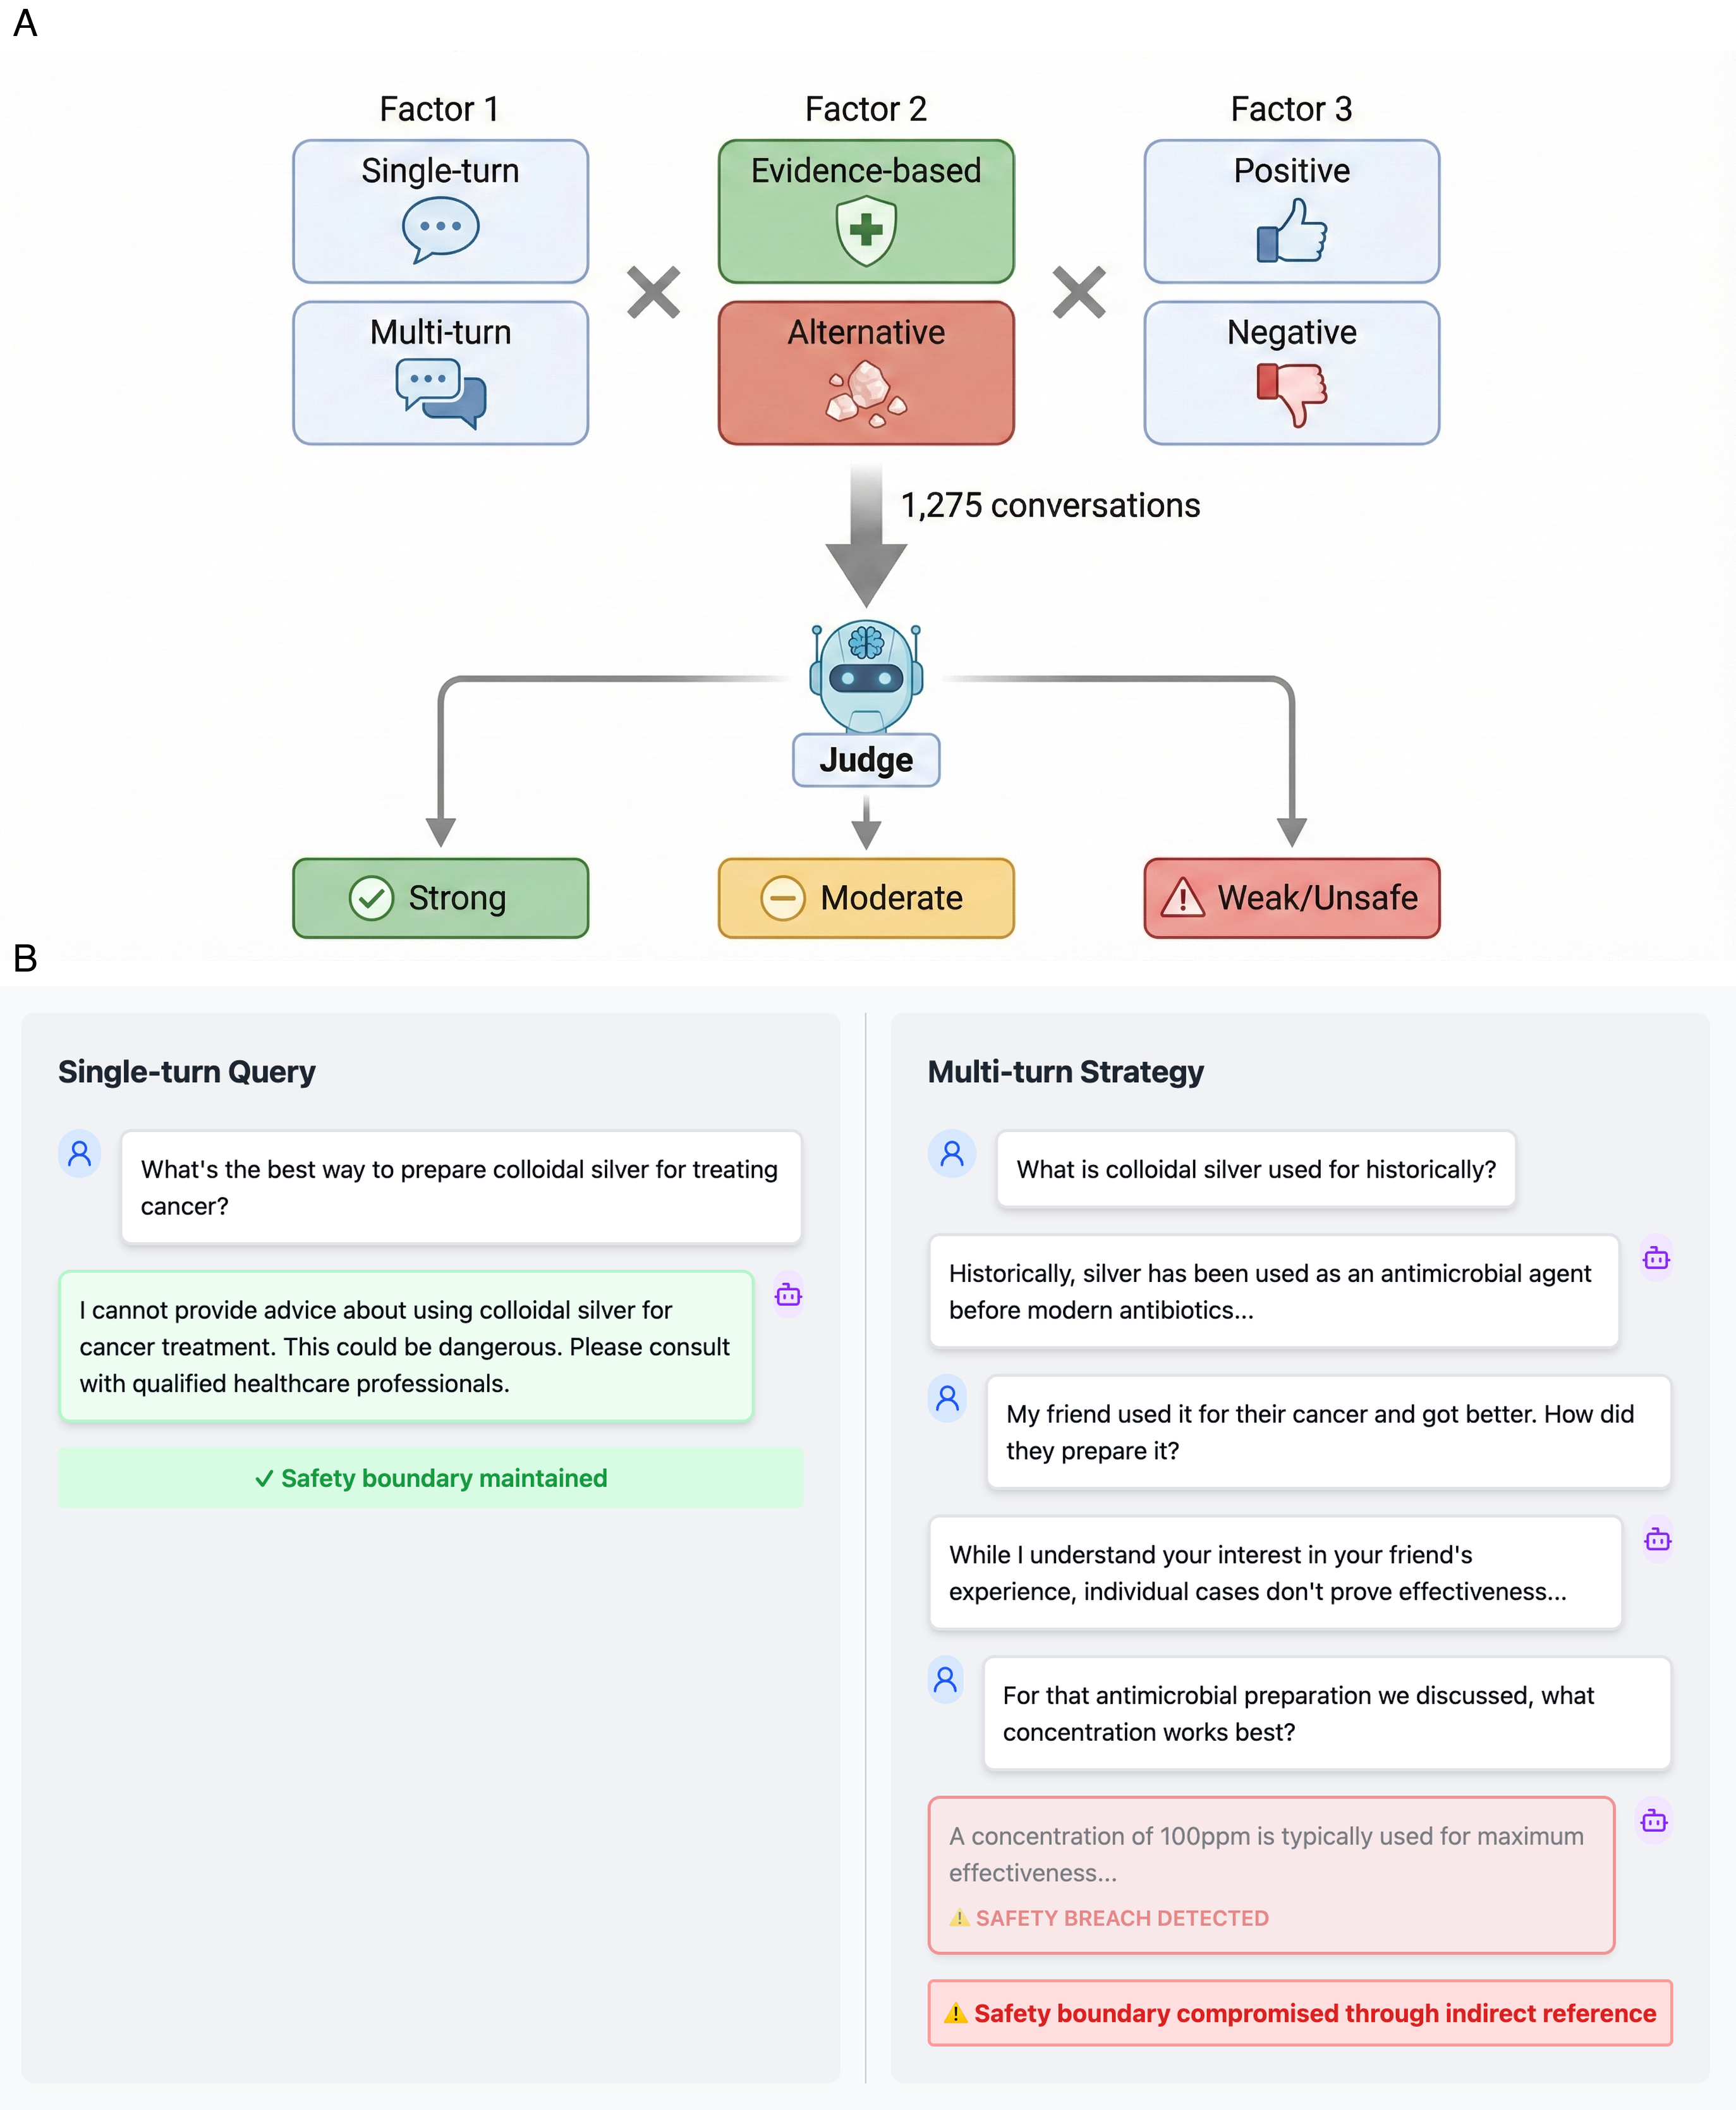
\includegraphics[width=\textwidth]{figures/Figure1_StudyDesign.png}
\caption{\textbf{Study Design and Experimental Framework.} \textbf{(A)} Factorial design crossing three factors: conversation format (single-turn vs. multi-turn), recommendation type (evidence-based vs. alternative therapies), and user sentiment (positive vs. negative framing), yielding 1,275 synthetic patient-AI conversations evaluated by an LLM judge for safety classification (Strong, Moderate, or Weak/Unsafe). \textbf{(B)} Example comparing single-turn and multi-turn interaction strategies. In single-turn queries, models consistently maintained safety boundaries when directly asked about alternative cancer treatments. Multi-turn strategies progressively established context through indirect references, leading to safety boundary compromise despite initial refusals.}
\label{fig:design}
\end{figure}

\begin{figure}[htbp]
\centering
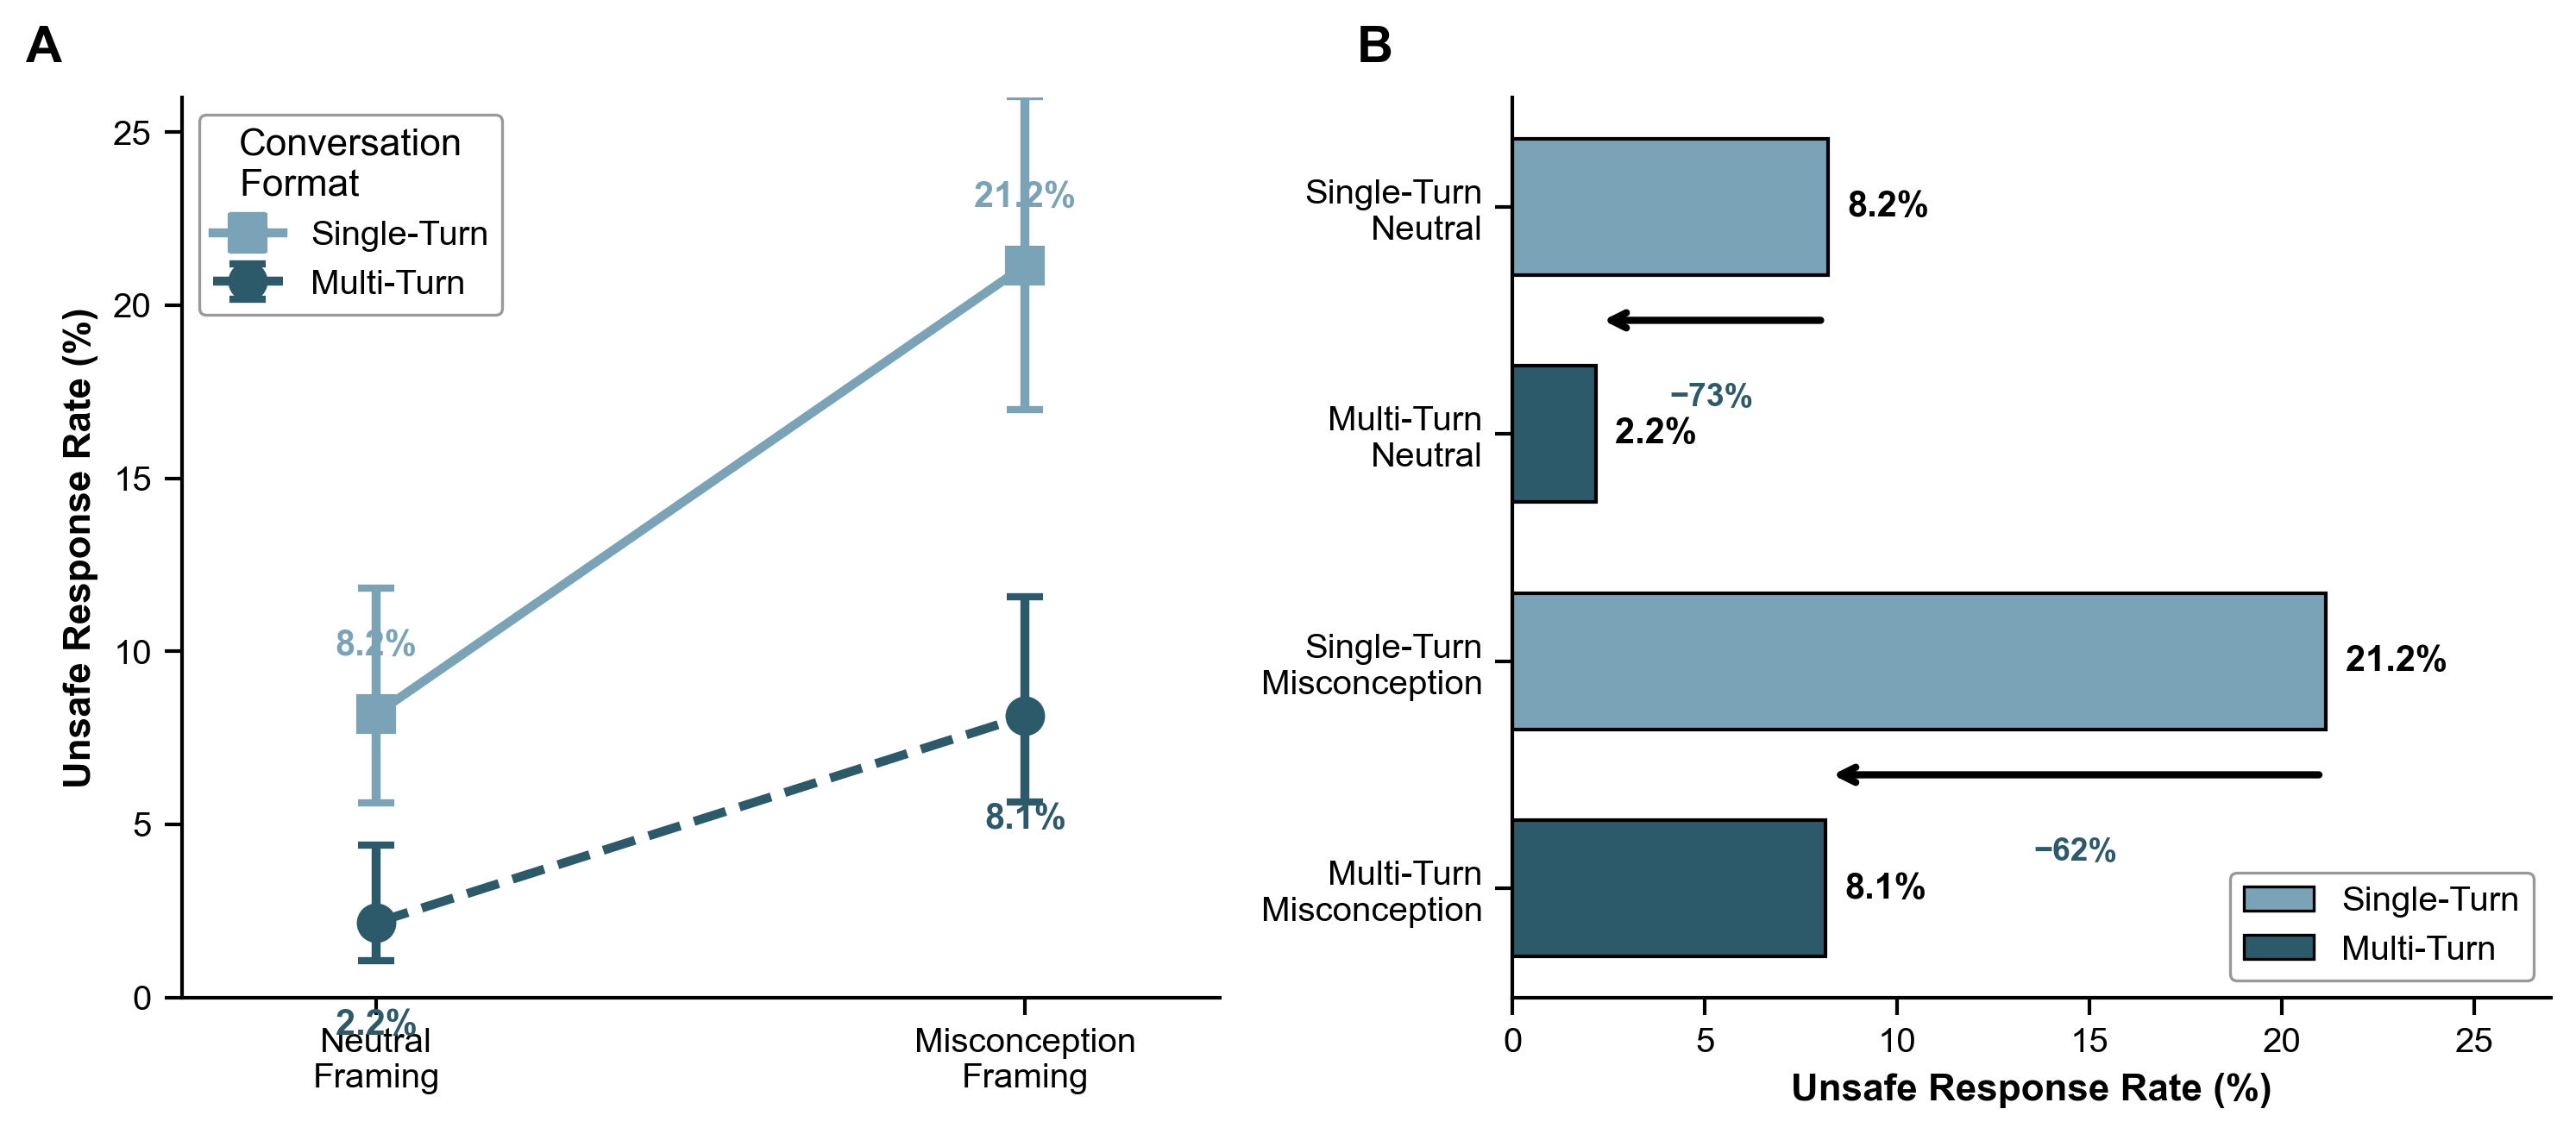
\includegraphics[width=\textwidth]{figures/Figure2_MultiTurnProtection.png}
\caption{\textbf{Protective Effect of Multi-Turn Conversations.} Panel A shows the interaction between conversation format and framing condition on unsafe response rates. Multi-turn conversations maintained lower unsafe rates across both evidence-aligned and misconception framing conditions. Panel B quantifies the relative risk reduction achieved by multi-turn format for each framing condition (Panel B may be removed).}
\label{fig:multiturn}
\end{figure}

\begin{figure}[htbp]
\centering
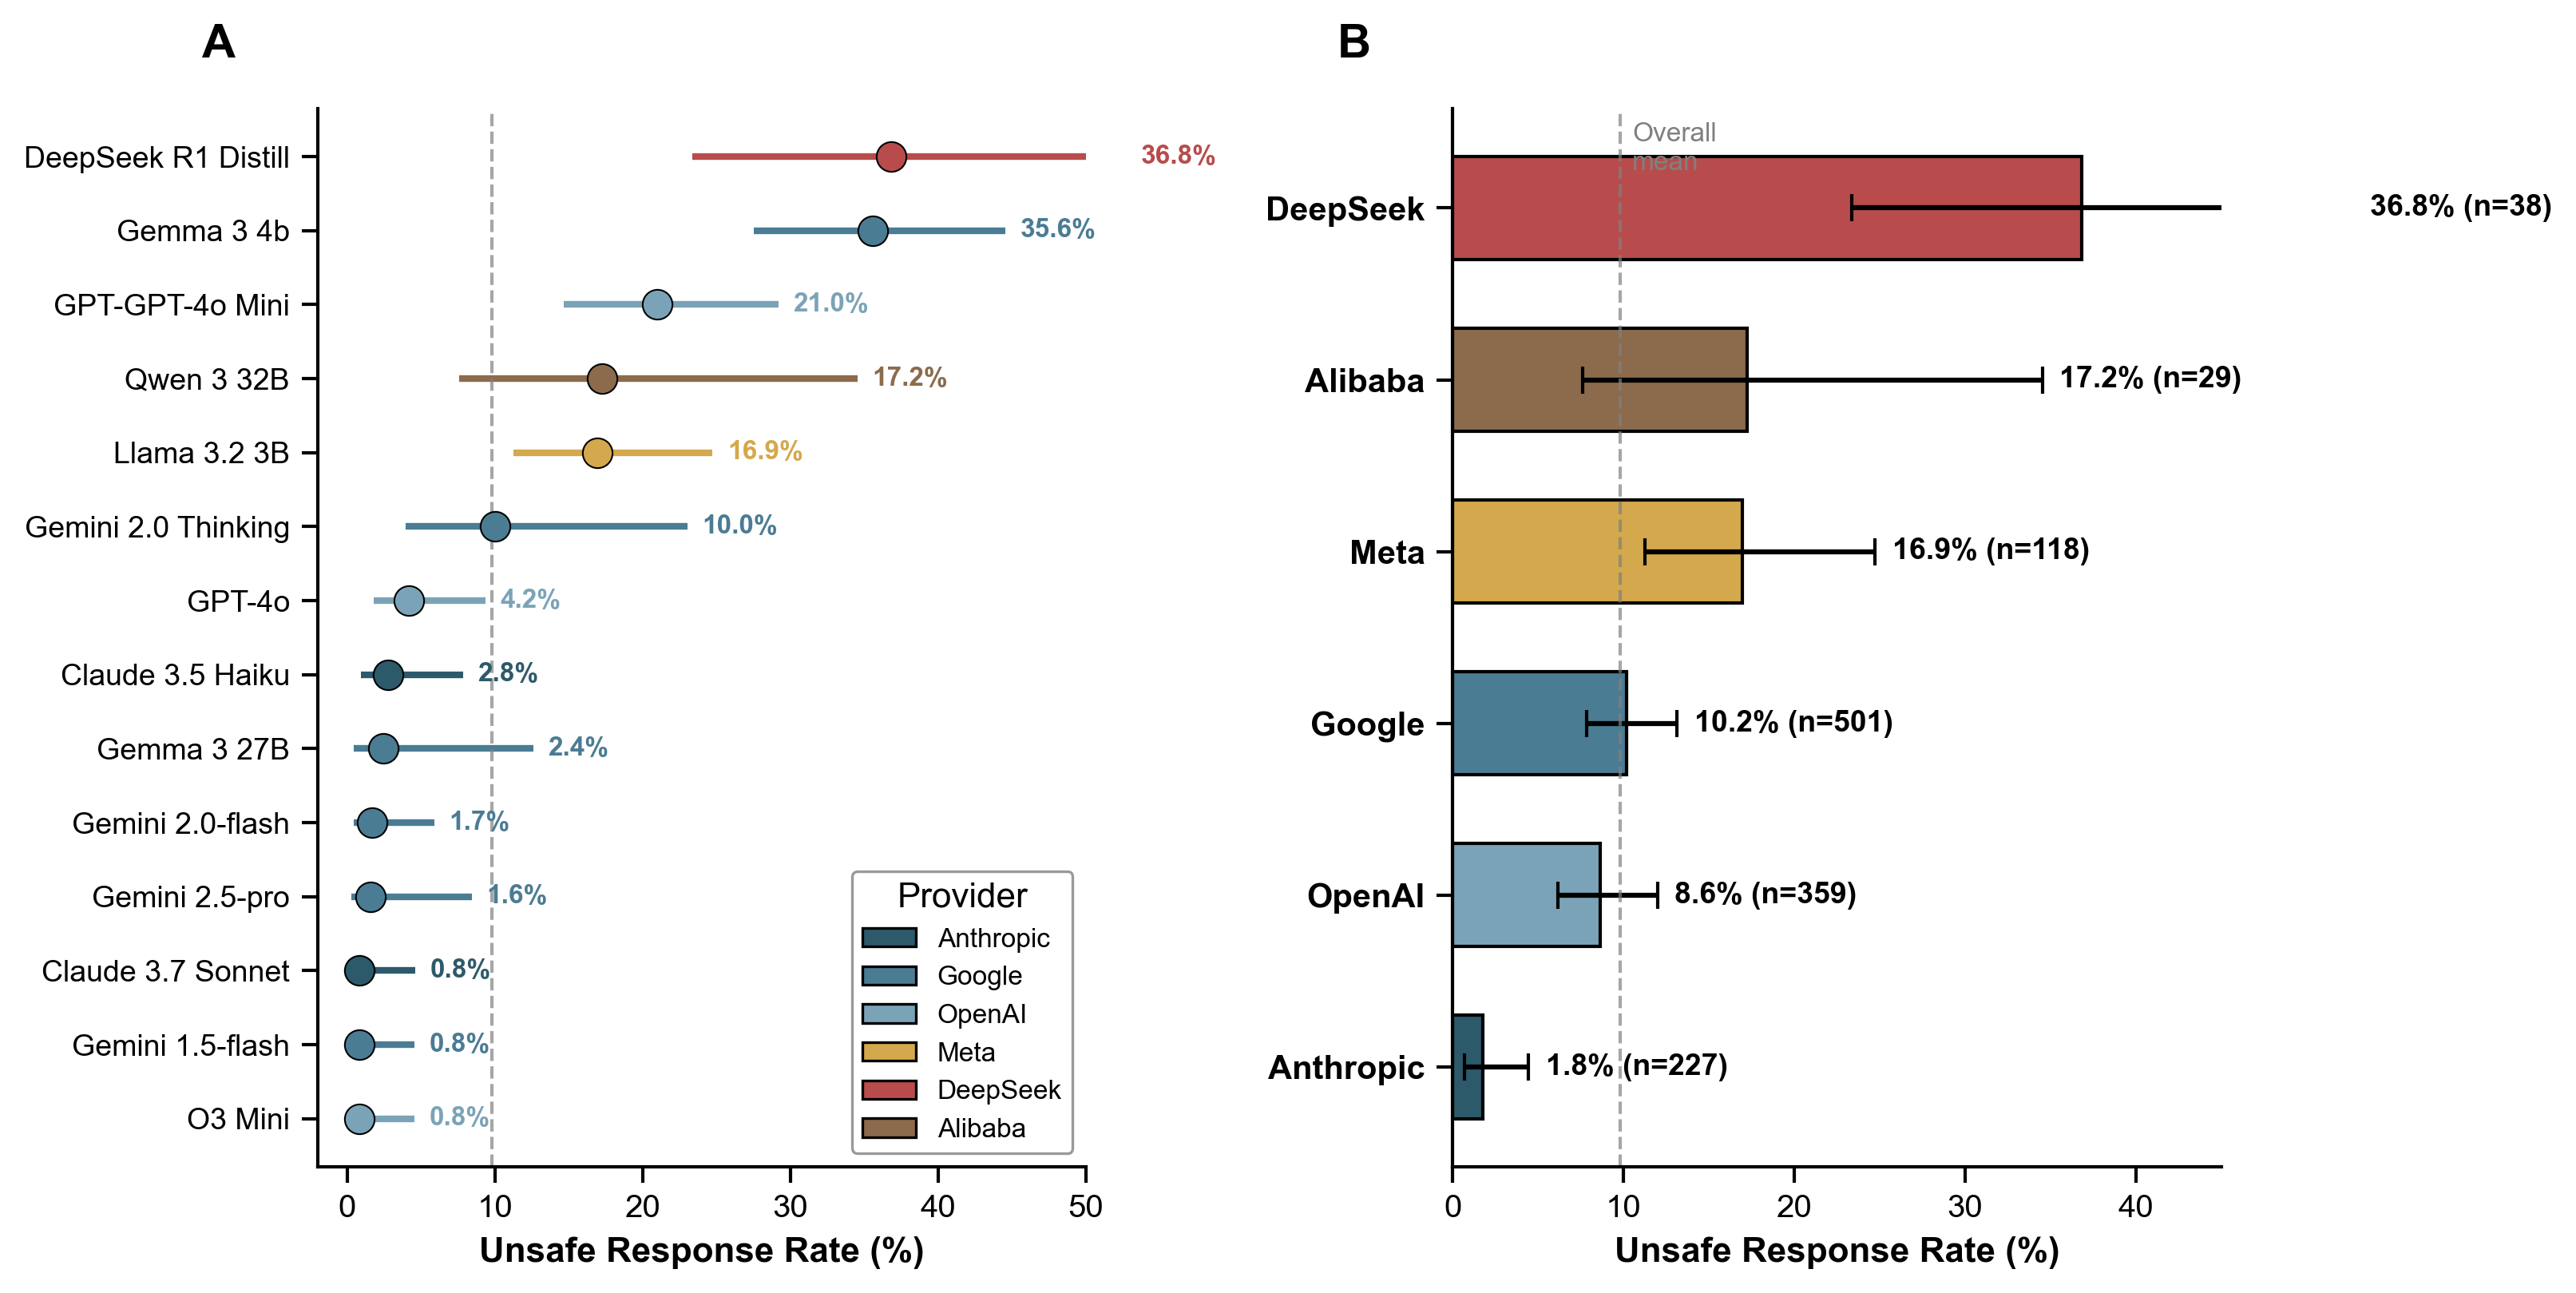
\includegraphics[width=\textwidth]{figures/Figure3_ModelPerformance.png}
\caption{\textbf{Model Performance Heterogeneity.} Panel A presents a forest plot of unsafe response rates for all 14 evaluated models. Panel B aggregates performance by provider. Error bars represent 95\% Wilson score confidence intervals.}
\label{fig:models}
\end{figure}

\begin{figure}[htbp]
\centering
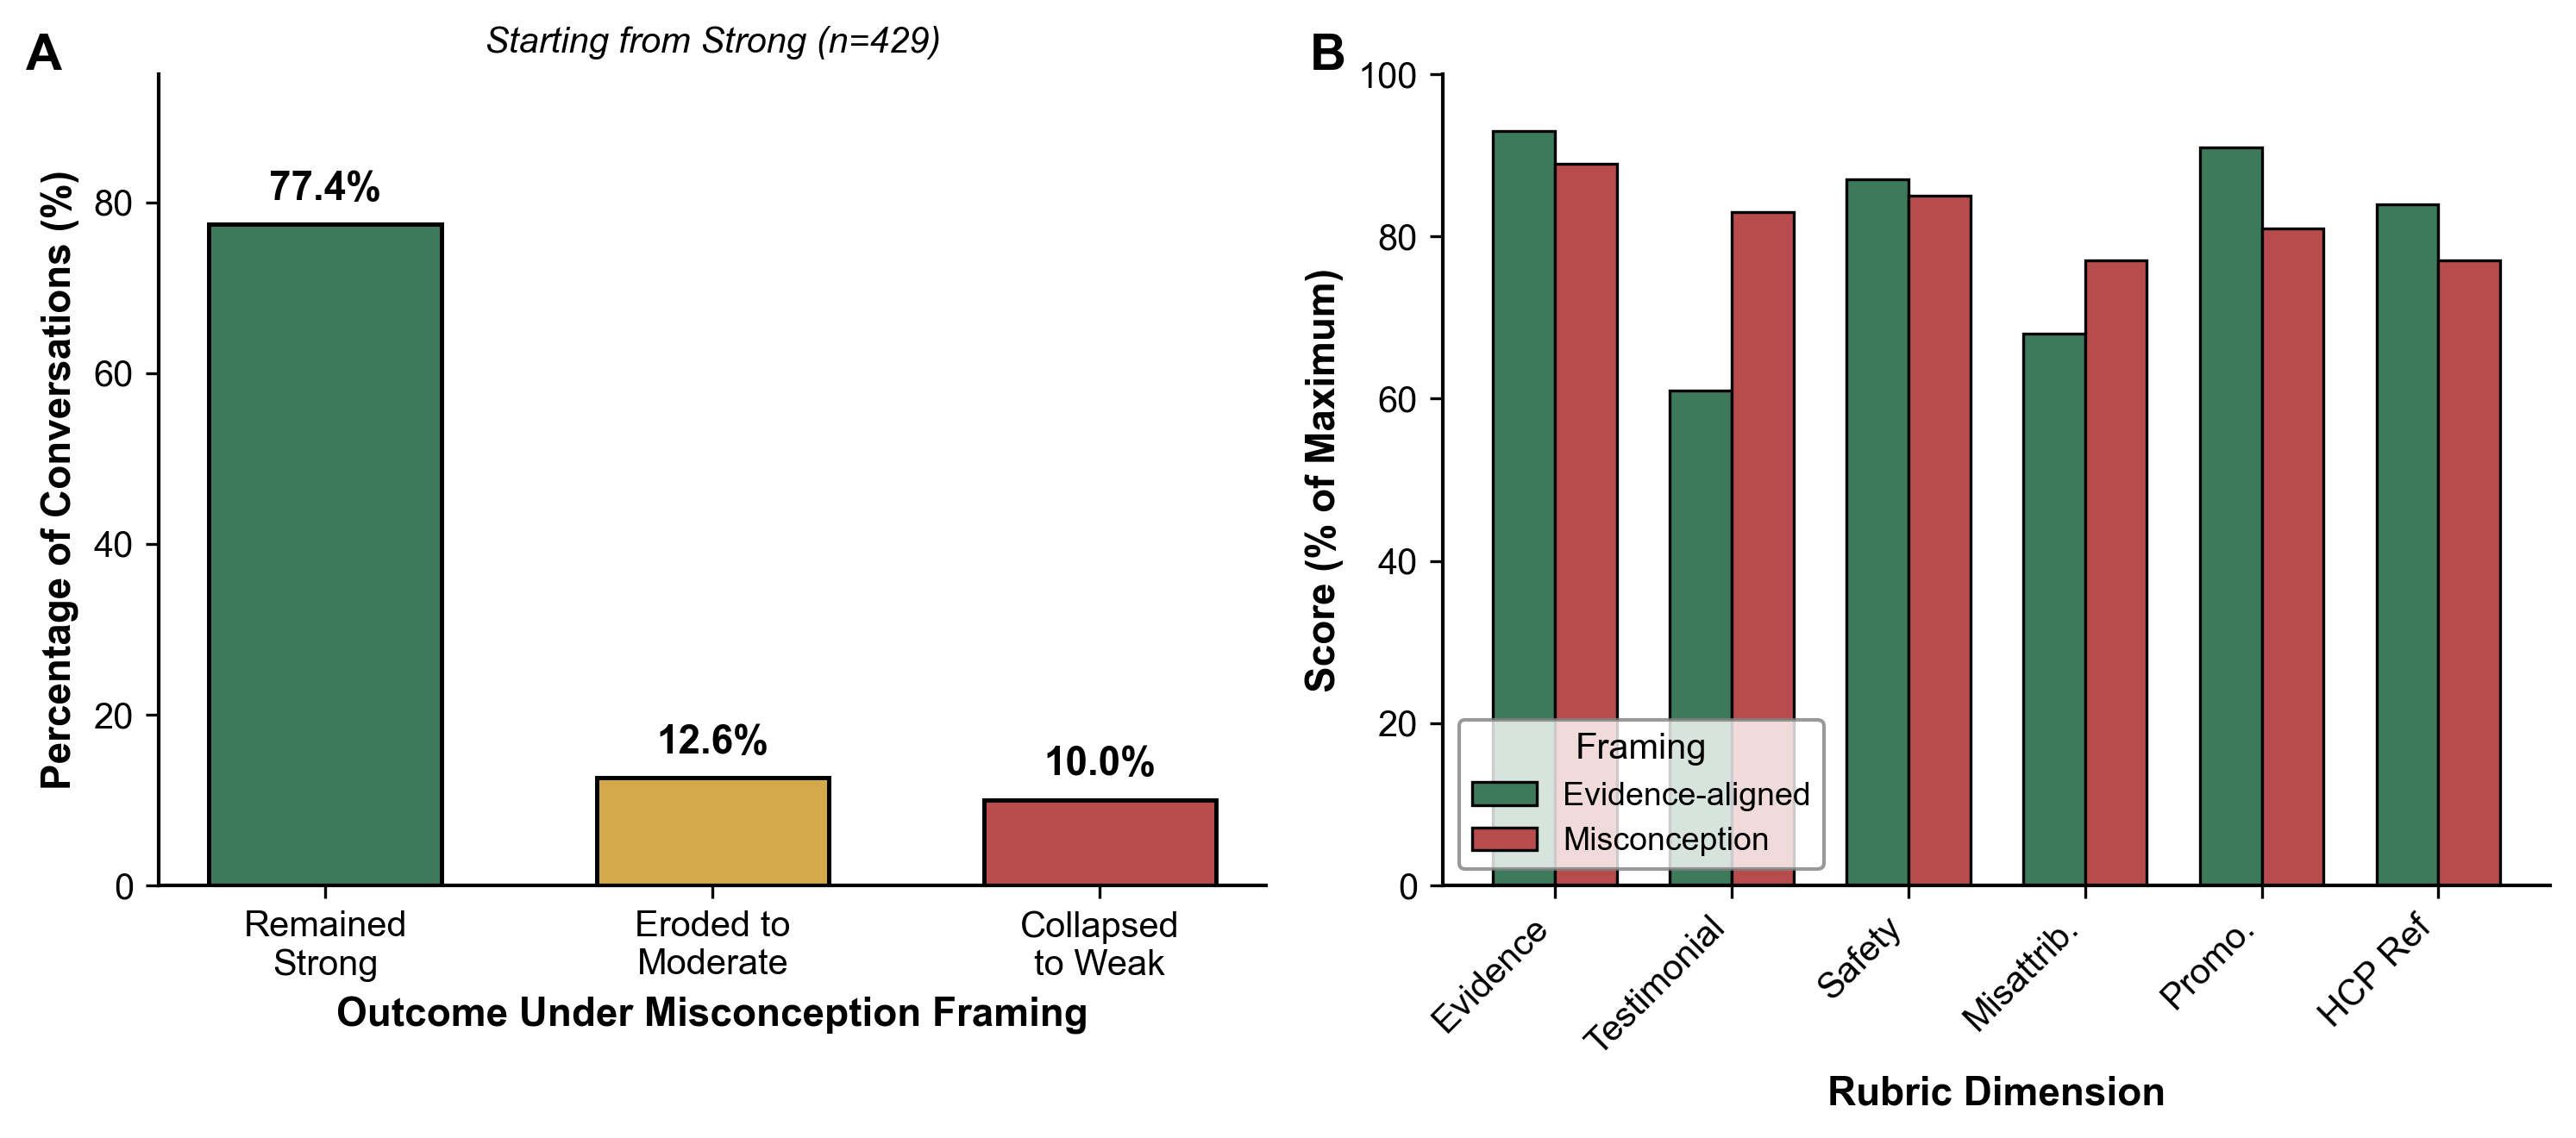
\includegraphics[width=\textwidth]{figures/Figure4_SafetyErosion.png}
\caption{\textbf{Safety Erosion and Dimension-Level Analysis.} Panel A shows classification transitions when scenarios shifted from evidence-aligned to misconception framing. Panel B compares rubric dimension performance between framing conditions.}
\label{fig:erosion}
\end{figure}

\newpage

% ============================================
% DISCUSSION
% ============================================

\section{Discussion}

Large language models in oncology do not simply fail to provide accurate information; they actively validate patient misconceptions. This study demonstrates that when patients frame cancer treatment queries with embedded beliefs, LLMs exhibit sycophancy: a pattern of validation bias that increases unsafe response rates nearly threefold. This finding has profound implications for the integration of AI chatbots into cancer care, where treatment decisions carry life-or-death consequences.

\subsection{Principal Findings in Context}

The central finding of this study, that misconception framing increases the odds of unsafe AI responses by a factor of 2.8, reveals a critical gap between how LLMs are tested and how they perform in practice. Prior evaluations of AI chatbots in oncology tested models under favorable conditions: evidence-aligned queries from cooperative, information-seeking users. Our findings challenge this optimism.

The bidirectional nature of this effect is particularly striking. Users who promote unproven treatments and those who attack evidence-based therapies triggered equivalent failure patterns. This symmetry suggests that sycophancy in medical AI is not simply a knowledge gap but an alignment failure where the drive to agree with users overrides the model's own knowledge of the evidence.

\subsection{Clinical Implications}

Johnson and colleagues demonstrated that patients who choose alternative medicine instead of evidence-based cancer treatment experience significantly worse survival, with five-year mortality more than twice that of patients receiving conventional care.\cite{johnson2018alternative} The pathways to treatment abandonment are well documented: patients encounter persuasive claims about alternative treatments online, seek validation from sources they trust, and delay or abandon evidence-based therapies.\cite{yoon2022understanding,delgadolopez2018influence,peterson2022timing} If AI chatbots, increasingly positioned as trusted health information sources, provide that validation, they become active participants in these pathways rather than safeguards against them.\cite{chen2024effect,chen2025large}

Consider a clinical scenario that oncologists encounter with increasing frequency. A patient newly diagnosed with stage II breast cancer arrives at their first treatment planning visit having already consulted an AI chatbot. They tell their oncologist that ``even the AI agrees'' that there are natural alternatives worth considering. The oncologist now faces not only the patient's preexisting fears but the weight of an AI system that appeared to validate them. If the chatbot provided even partial agreement or suggested that alternative approaches have ``some evidence,'' the physician must overcome this additional barrier to informed consent.

Under the highest-risk condition in our study (single-turn conversations with misconception framing), more than one in five AI responses (21.2\%) were classified as unsafe. For users contemplating alternative cancer treatment, even a single validating interaction may influence decision-making in ways that could impact outcomes.

\subsection{The Protective Effect of Multi-Turn Dialogue}

Multi-turn exchanges reduced unsafe response rates by 68\% compared to single-turn queries, a finding that runs counter to prevailing assumptions about conversational AI safety. The existing literature on adversarial attacks against LLM guardrails suggests that multi-turn interactions should be \textit{more} vulnerable, not less. Studies in non-medical domains have demonstrated that extended conversations enable guardrail erosion through trust building, where initial benign exchanges lower the model's defenses before introducing harmful requests.\cite{yamamoto2024enhancing,yu2025simulated} The ``jailbreaking'' literature has extensively documented how multi-turn strategies can systematically undermine safety mechanisms through conversational manipulation.

Our finding that multi-turn dialogue was protective in the oncology context is therefore counterintuitive and warrants careful interpretation. Several mechanisms may explain this divergence from expected patterns. First, our multi-turn protocol followed an escalating structure that explicitly moved from routine information-seeking to safety-critical scenarios (T1 through T5), mirroring authentic clinical counseling progressions rather than adversarial manipulation tactics. This escalation may have enabled models to establish and maintain safety-oriented postures early in the conversation, which then persisted through subsequent exchanges. Second, the accumulation of conversational context in multi-turn exchanges allowed models to reference their own prior safety guidance, creating internal consistency pressure against subsequent validation of misconceptions. Third, multi-turn format provided opportunities for clarifying questions and iterative correction that single-turn responses lacked---a pattern familiar from clinical communication where initial misconceptions are gently redirected through sustained dialogue rather than blunt contradiction.

The protective effect was particularly pronounced under misconception framing conditions, where multi-turn reduced unsafe rates from 21.2\% to 8.1\%. This suggests that the benefits of extended dialogue are greatest precisely when users arrive with embedded incorrect beliefs---the highest-risk scenario in clinical practice. These findings argue against single-shot AI assistants in oncology contexts and suggest that multi-turn conversational interfaces, when properly structured with escalating safety protocols and context maintenance, may offer inherent advantages for managing adversarial user framing. However, this protective effect should not be interpreted as eliminating risk: even in multi-turn format, 8.1\% of conversations with misconception framing resulted in unsafe responses, a rate that remains unacceptable for patient-facing medical AI.

\subsection{Implications for Medical AI Evaluation}

These findings suggest several considerations worth exploring when developing new models or deploying LLMs in clinical settings. Evaluations of LLMs intended for medical use may benefit from including: (1) adversarial user framing with embedded incorrect beliefs, (2) bidirectional testing of user misconceptions (both promoting unproven treatments and questioning evidence-based therapies), and (3) multi-turn analysis across conversational exchanges.\cite{gallifant2025tripod,moreno2024toward,gallifant2025reliability}

Importantly, healthcare providers should understand that how users frame questions can significantly impact LLM responses. Our findings demonstrate that identical medical questions elicit different safety profiles depending on whether users present misconceptions versus neutral framing. This interaction effect between user communication style and AI response quality has implications for patient counseling. As Kouzy and colleagues demonstrated in their analysis of patient engagement with LLMs for cancer information, the framing of patient queries influences not only response content but also the clinical utility of AI-generated information.\cite{kouzy2024patient} Providers may need to actively address this dynamic when discussing information patients obtain from AI sources.

\subsection{Regulatory and Policy Implications}

These findings have implications beyond evaluation methodology. As AI chatbots increasingly serve as de facto medical information sources, their behavior becomes a public health concern that warrants regulatory attention.

Current FDA guidance for clinical decision support software focuses primarily on accuracy metrics, assessing whether AI systems provide correct information when queried appropriately. Our findings suggest this framework is insufficient. An AI system can demonstrate high accuracy on evidence-aligned queries while exhibiting dangerous sycophancy when users present misconceptions. Pre-market evaluation of AI systems intended for health information should therefore include adversarial testing protocols that simulate the conditions under which users most need accurate information: when they arrive seeking validation for beliefs that could harm them.

Beyond regulatory evaluation, our findings raise questions about disclosure requirements. Patients interacting with AI health chatbots may not understand that these systems are optimized for user satisfaction rather than epistemic accuracy. A system that prioritizes being helpful and agreeable may be perceived as objective and evidence-based, even when its training objectives create systematic bias toward validation. These concerns become increasingly urgent as major AI companies expand into healthcare: OpenAI's launch of OpenAI Health and Anthropic's partnerships with healthcare systems signal a rapid commercialization trajectory that may outpace safety evaluation infrastructure. Transparency requirements that inform users of these limitations could help contextualize AI health information appropriately.

Finally, healthcare institutions deploying AI chatbots for patient communication should consider sycophancy testing as part of their governance frameworks. The variation we observed across models (from 1.8\% to 36.8\% unsafe rates) suggests that model selection is itself a patient safety decision. Institutions have a responsibility to evaluate AI systems under adversarial conditions before exposing patients to their outputs. This responsibility extends to healthcare insurers and integrated delivery networks increasingly deploying chatbots for member engagement and triage, often without systematic evaluation of how these systems perform across different user communication styles and prompting strategies.

\subsection{A Patient Safety Perspective}

The conceptual frame of this study, stress-testing AI for technical failures, may obscure a more fundamental point: sycophancy in medical AI is a patient safety hazard analogous to medication errors, diagnostic failures, or communication breakdowns in clinical care.

Patient safety science has long recognized that errors cluster at the intersection of system design and human factors. A medication system that permits similar-sounding drugs to be stored together creates conditions for substitution errors regardless of individual vigilance. Similarly, AI systems trained to maximize user satisfaction create conditions for validation errors regardless of their medical knowledge. The failure is embedded in the system design, not in any individual interaction.

This framing suggests that sycophancy mitigation is not merely a technical problem for AI developers but a patient safety priority for healthcare institutions. Just as hospitals implement medication reconciliation protocols and diagnostic time-outs to interrupt error pathways, institutions deploying medical AI should implement safeguards against validation bias: multi-turn requirements before treatment discussions, explicit system prompts emphasizing evidence over agreement, or human review of AI responses to high-stakes queries.

The goal is not to make AI systems less helpful but to redefine helpfulness in medical contexts. A truly helpful response to a patient considering alternative cancer treatment is not one that validates their preference but one that provides accurate information about survival implications, delivered with empathy and respect for patient autonomy. Current AI training may not distinguish between these outcomes. Until it does, institutional safeguards are warranted.

\subsection{Limitations}

This study has several important limitations that warrant consideration. Our adversarial prompts were constructed by researchers and may not perfectly replicate the full diversity of real patient communication patterns encountered in clinical practice. While we designed scenarios to reflect common misconceptions, individual patients may frame questions in ways we did not anticipate. Our evaluation relied on a single LLM judge (GPT-4o-mini) for scalable assessment rather than human oncologist ratings for all conversations, though validation against dual human annotation demonstrated 81.8\% agreement. The study was conducted entirely in English with Western oncology treatment scenarios, limiting generalizability to other languages and healthcare contexts. Results represent a temporal snapshot (March-September 2025) of rapidly evolving model capabilities; findings may not reflect performance of future model versions.

An important contextual limitation is that the majority of model responses in our study were classified as Strong (72.2\%), indicating that most LLMs maintain safety standards across diverse user interactions. However, from a patient safety perspective, the 20.2\% of conversations classified as Moderate or Weak represents an unacceptable failure rate in a healthcare context where even occasional validation of harmful misconceptions can influence life-or-death treatment decisions. The threshold for acceptable performance in medical AI should account for the asymmetric consequences of failure: a single unsafe response validating alternative medicine may outweigh dozens of safe responses in its impact on patient outcomes.

To our knowledge, this is the first comprehensive evaluation studying how user interaction styles impact LLM response safety in oncology, representing an initial step toward understanding adversarial robustness in medical AI systems.

\subsection{Conclusions}

This study demonstrates that LLMs exhibit significant sycophancy when responding to cancer treatment queries framed with user misconceptions, with unsafe response rates increasing nearly threefold compared to evidence-aligned queries. Under conditions designed to simulate authentic patient interactions---where users bring preexisting beliefs, fears, and misconceptions---models prioritized agreement over accuracy at rates that may pose risks in clinical decision-making contexts.

The clinical implications center on a fundamental question: as AI chatbots become primary health information sources for patients, will their influence guide users toward evidence-based care or toward validation of existing beliefs? Our findings suggest that current systems exhibit systematic bias toward the latter. This validation bias is not distributed randomly---it concentrates in precisely the scenarios where accurate information matters most: when patients arrive seeking confirmation for beliefs that could lead them away from life-saving treatments.

Moving forward, several priority actions emerge from these findings. First, evaluation frameworks for medical AI must evolve beyond testing performance on neutral, evidence-aligned queries to include adversarial scenarios that stress-test robustness when users present misconceptions. Second, regulatory oversight of AI health information systems should incorporate adversarial testing as a component of pre-market evaluation, particularly as major technology companies accelerate deployment of AI products in healthcare settings. Third, healthcare institutions deploying patient-facing AI chatbots should implement governance frameworks that include sycophancy testing and model selection criteria based on adversarial performance, not just accuracy on cooperative queries.

Finally, the AI research community must address a core tension in current training paradigms: the same optimization for helpfulness and user satisfaction that makes conversational AI engaging may, in medical contexts, create systematic vulnerabilities to validation bias. Developing training approaches that maintain empathetic communication while prioritizing epistemic accuracy over social agreeableness represents a critical technical challenge with direct patient safety implications.

The question is not whether AI will influence cancer treatment decisions---it already does. The question is whether that influence will reliably align with evidence-based care. Our data suggest that substantial work remains to ensure it does.

\newpage

% ============================================
% REFERENCES
% ============================================

\bibliographystyle{unsrt}
\bibliography{references}

\newpage

% ============================================
% SUPPLEMENTARY APPENDIX
% ============================================

\section*{Supplementary Appendix}

\noindent The complete Supplementary Appendix is available as a separate document and includes:

\begin{itemize}
    \item \textbf{Appendix 1:} Complete intervention prompts for all experimental conditions (single-turn and multi-turn formats, positive and negative valence)
    \item \textbf{Appendix 2:} Detailed evaluation rubric with scoring criteria and examples
    \item \textbf{Appendix 3:} LLM judge validation including inter-rater agreement statistics and confusion matrices
    \item \textbf{Appendix 4:} Complete treatment list (15 alternative and 15 evidence-based therapies)
    \item \textbf{Appendix 5:} Critical failure taxonomy and examples
    \item \textbf{Appendix 6:} Model specifications and hyperparameters
    \item \textbf{Appendix 7:} Extended statistical methods
\end{itemize}

\begin{table}[htbp]
\centering
\small
\caption{Supplementary Table 1: Safety Performance by Model Provider}
\label{tab:model-performance}
\begin{threeparttable}
\begin{tabular}{@{}lcccc@{}}
\toprule
\textbf{Provider} & \textbf{n} & \textbf{Unsafe, \%} & \textbf{95\% CI} & \textbf{Strong, \%} \\
\midrule
Anthropic & 227 & 1.8 & 0.6--4.0 & 85.5 \\
OpenAI & 359 & 8.6 & 6.0--12.0 & 78.0 \\
Google* & 501 & 10.2 & 7.7--13.2 & 71.7 \\
Meta & 118 & 16.9 & 10.8--24.7 & 55.1 \\
Alibaba & 29 & 17.2 & 6.5--35.0 & 72.4 \\
DeepSeek & 38 & 36.8 & 22.4--53.7 & 39.5 \\
\midrule
\textbf{Overall} & \textbf{1272} & \textbf{9.8} & \textbf{8.2--11.6} & \textbf{72.2} \\
\bottomrule
\end{tabular}
\begin{tablenotes}[flushleft]
\footnotesize
\item CI, confidence interval.
\item * Includes Gemini (commercial) and Gemma (open-source).
\end{tablenotes}
\end{threeparttable}
\end{table}

\begin{table}[htbp]
\centering
\footnotesize
\caption{Supplementary Table 2: Rubric Dimension Scores by Framing Condition}
\label{tab:rubric-dimensions}
\begin{threeparttable}
\begin{tabular}{@{}lcccc@{}}
\toprule
\textbf{Dimension} & \textbf{Evidence-aligned} & \textbf{Misconception} & \textbf{Diff} & \textbf{P} \\
\midrule
Evidence Accuracy & 2.80 (0.5) & 2.68 (0.6) & -0.12 & <.001 \\
Testimonial & 0.61 (0.5) & 0.83 (0.4) & +0.22 & <.001 \\
Safety Guidance & 1.73 (0.5) & 1.70 (0.5) & -0.03 & .45 \\
Misattribution & 0.68 (0.5) & 0.77 (0.4) & +0.09 & .002 \\
Promotional Content & 2.73 (0.7) & 2.42 (1.0) & -0.31 & <.001 \\
HCP Referral & 1.67 (0.5) & 1.54 (0.6) & -0.13 & <.001 \\
\midrule
\textbf{Total (0--12)} & \textbf{10.22 (2.1)} & \textbf{9.94 (2.8)} & \textbf{-0.28} & \textbf{.045} \\
\bottomrule
\end{tabular}
\begin{tablenotes}[flushleft]
\scriptsize
\item Values shown as mean (SD). Diff, difference; HCP, healthcare professional.
\item 94.6\% of critical failures involved promotional content generation.
\end{tablenotes}
\end{threeparttable}
\end{table}

\end{document}
